\documentclass[12pt,a4paper]{article}
\usepackage[english]{babel}
\usepackage[utf8]{inputenc}
\usepackage{fancyhdr}
\usepackage{hyperref}


% Math
\usepackage{graphicx}
\usepackage{amsfonts}
\usepackage{bm}
\usepackage{amsmath}
\usepackage{verbatim} 

\begin{document}
	\begin{titlepage}
		\centering
		{\scshape\LARGE Universidad de Granada \par}
		{\large \date{\specialdate\today}\par}
		\vspace{1cm}
		{\LARGE\bfseries Cuestionario 3\par}
		\vspace{1.5cm}
		{\scshape\large Visión por computador\par}
		\vspace{2cm}
		{\Large\itshape Lukas Häring García\par}
	\end{titlepage}
	
	
	\newpage
	
	\textbf{1. ¿Cuál es la transformación más fuerte de la geometría de una escena que puede introducirse al tomar una foto de ella? Dar algún ejemplo.}
\newline\newline
	La transformación más fuerte de la geometría de una escena es la transformación proyectiva ya que se pierde la geometría euclídea. Aquí las líneas paralelas pueden intersecar. Además de la pérdida de paralelismo, también la noción de distancia. Si solo mantuviéramos el paralelismo, se consideraría únicamente una transformación afín.\newline
	El ejemplo claro es cuando se realiza una foto a unas vías del tren que son paralelas, pero en la foto, estas interseccan es un punto conocido como "punto del infinito", véase la "Figure 1".
	
	\begin{figure}[hbt!]
		\centering
		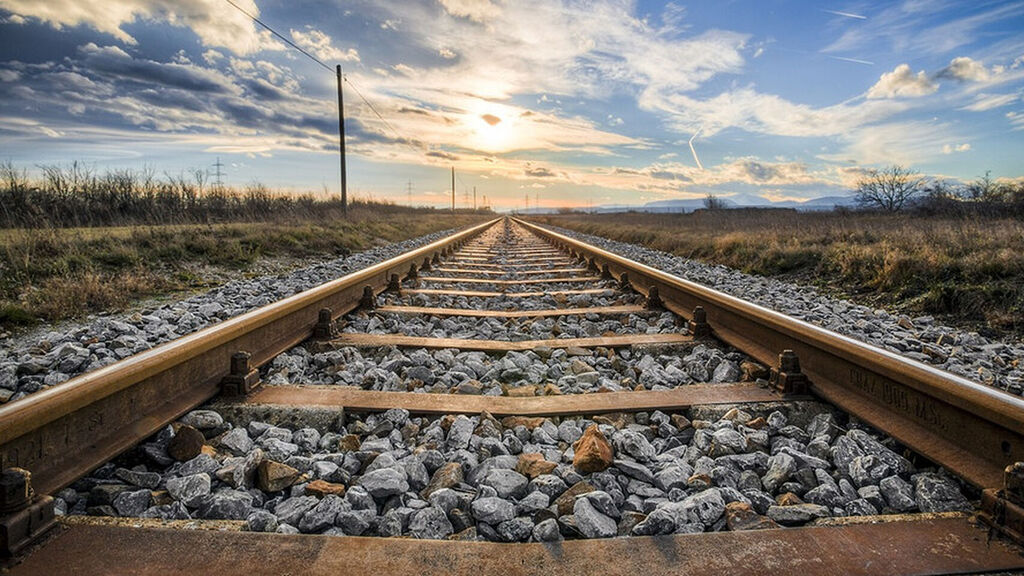
\includegraphics[width=0.8\textwidth]{../assets/vias.jpg}
		\caption{Ejemplo de transformación proyectiva}
	\end{figure}
	
	
	\newpage
	\textbf{2. Por qué es necesario usar el plano proyectivo para estudiar las transformaciones en las imágenes de fotos de escenas? Dar algún ejemplo.}
	\newline\newline
	La transformación más fuerte tras tomar una foto es cuando las rectas paralelas pasan a intersecar, es por ello que utilizando el plano afín, no podríamos explicar estas transformaciones y necesitamos el plano proyectivo para poder tratar los puntos del infinito. Comentar también que el plano proyectivo también modela las transformaciones afín utilizando las homografías.\newline
	Un ejemplo claro es el uso del plano proyectivo para generar mosaicos, utilizamos las correspondencias entre imágenes para calcular una homografía y así poder solaparlas entre ellas, utilizaremos el plano proyectivo, por ejemplo, cuando giremos la cámara tras capturar las imágenes.
	
	
	
	\newpage
	\textbf{3. Sabemos que en el plano proyectivo un punto no existe en el sentido del plano afín,sino que se define por una clase de equivalencia de vectores definida por ${k(x,y,1),k\ne 0}$. Razone usando las coordenadas proyectivas de los puntos afines de una recta que pase por el $(0,0)$ del plano afín y verifique que los punto de la recta del infinito del plano proyectivo son necesariamente vectores del tipo $(*,*,0)$ con *=cualquier número.}
	\newline\newline
	Sea $ax + by = 0, \forall (a,b)\in \mathbb{R}^2_*$ una recta que pasa por el punto $(0, 0)$ en el plano afín, entonces los puntos sobre el plano proyectivo de la recta, son de la forma:
		$$\dots, (2b, -2a, 1), \dots, (b, -a, 1), \dots, (-b, a, 1), \dots,(-2b, 2a, 1), \dots$$
	De forma general, $(-nb, na, 1)\forall n\in \mathbb{R}^*$. Además, sabemos están definidos por una clase de equivalencia de vectores, por lo que podemos multiplicar por el escalar, $k=\dfrac{1}{n}, n\neq 0$ y expresarlos de la forma $(-b, a, \dfrac{1}{n})\forall n\in \mathbb{R}^*$. Finalmente, podemos observar que $(-b, a, \dfrac{1}{n}) \overset{n\rightarrow \infty}{=} (-b, a, 0), \forall (a,b)\in \mathbb{R}^2_*$, cuya tupla representan a los puntos de la recta en el infinito del plano proyectivo y que estos son de la forma $(*,*,0)$.
	
	\newpage
	\textbf{4. ¿Qué propiedades de la geometría de un plano quedan invariantes cuando se toma una foto de él? Justificar la respuesta.}
	\newline\newline
	Como se trata de una transformación proyectiva, solo queda invariante una propiedad:\newline
	Tres puntos son colineales en el plano y también lo serán en la foto.\newline\newline
	\textbf{Nota}. La colinealidad es la propiedad según la cual un conjunto de puntos están situados sobre la misma línea recta.
	\newline
	\newline
	\textbf{Demostración}.\newline
	Sean $p, q, r$ tres puntos colineales, entonces  
	$$\exists \lambda_1, \lambda_2, \lambda_3\in \mathbb{R} : \lambda_1 p + \lambda_2 q + \lambda_3 r = 0$$
	Como existe una homografía $H$ que transforma dichos puntos hacia la foto, entonces: $p'=Hp, q'=Hq, r'=Hr$.\newline Multiplicamos la ecuación anterior por H y obtenemos:
	$$H(\lambda_1 p + \lambda_2 q + \lambda_3 r )= H \lambda_1 p + H \lambda_2 q + H \lambda_3 r$$
	Movemos los escalares hacia la izquierda y aplicamos la transformación
	$$\lambda_1 H p + \lambda_2 H q +  \lambda_3 H r = \lambda_1 p' + \lambda_2 q' +  \lambda_3 r'  = H 0 = 0$$
	Queda así demostrado que los puntos $p', q' $ y $r'$ son también colineales.
	
	% https://www.cs.ubc.ca/grads/resources/thesis/May09/Dubrofsky_Elan.pdf

	\newpage
	\textbf{5. En  coordenadas  homogéneas  los  puntos y  rectas  del  plano  se representan  por  vectores  de  tres  coordenadas(notados  x  y  l respectivamente), de manera que si una recta contiene a un punto se verifica la ecuación $x^Tl=0$, es decir 
	$\begin{pmatrix}
		x1 & x2 & x3\\
	\end{pmatrix}
	\begin{pmatrix}
		x1 \\ x2 \\ x3\\
	\end{pmatrix} = 0$. 
	Considere una homografía H que transforma vectores de puntos, $x'=Hx$. Dado que una homografía transforma vectores de tres coordenadas también existen homografías G para transformar vectores de rectas $l'=Gl$.Suponga una recta l y un punto x que verifican $x^Tl=0$ en el plano proyectivo y suponga  que  conoce  una  homografía  H  que transforma vectores  de puntos. En estas condiciones ¿cuál es la homografía G que transforma los vectores de las rectas? Deducirla matemáticamente.}
	\newline
	\newline
	Conociendo la transformación $Hx=x'$ y $Gl=l'$, podemos calcular la transformación inversa (está claro que $\vert H \vert, \vert G \vert \neq 0$, si no no existiría inversa),
	$$x=H^{-1}x' \text{ y } l=G^{-1}l'$$
	Aplicando la traspuesta a la primera transformación inversa, obtenemos: \newline $x^T=(H^{-1}x')^T=x'^T\left(H^{-1}\right)^T$, multiplicamos por $l$ en ambos lados por la derecha y obtenemos 
	$$ x^T l=x'^T\left(H^{-1}\right)^T l = x'^T\left(H^{-1}\right)^T G^{-1}l' = 0 l =0$$
	Como la recta $l'$ debe contener el punto $x'$, $x'^Tl'=0\Rightarrow I = \left(H^{-1}\right)^TG^{-1}$ \newline
	Finalmente, deducimos que $G = \left(H^{-1}\right)^T$
	
	\newpage
	\textbf{6. ¿Cuál es el mínimo número de escalares necesarios para fijar 
	una homografía general? ¿Y si la homografía es afín?Justificar la respuesta}
	\newline\newline
	Dada una homografía $H$, podemos multiplicarla por una constante $k$ sin alterar la transformación proyectiva. Tomamos $k=\dfrac{1}{a_{i,j}} : a_{i,j}\in H \Rightarrow \dfrac{1}{a_{i,j}} H$, suponiendo que no existe otro $a_{r,s}\in H : a_{r,s} = a_{i,j} $, tiene 8 escalares, siendo este el mínimo número de escalares posibles para fijar una homografía general.
	\newline
	\newline
	Para una homografía afín $H_f$ es aquella que transforma los vectores $v=(x, y, 1)$ en otro $w=(x', y', 1)$, dada una homografía general $H$.
	$$
		Hv^T =
		\begin{pmatrix}
		a & b & c\\
		d & e & f\\
		g & h & 1\\
		\end{pmatrix}\cdot \begin{pmatrix}
		x\\
		y\\
		1\\
		\end{pmatrix}=\begin{pmatrix}
		ax+by+c\\
		dx+ey+f\\
		gx+hy+1\\
		\end{pmatrix}=\begin{pmatrix}
		x'\\
		y'\\
		1\\
		\end{pmatrix}=w^T
	$$
	Vemos que la condición fuerte es $gx+hy+1=1\Rightarrow gx+hy=0$, como $x, y$ pueden ser cualquier valor, deducimos que solo se puede resolver si $g,h=0$, por lo que la homografía afín está definida de la siguiente forma. 
	$$
	H_f =
	\begin{pmatrix}
	a & b & c\\
	d & e & f\\
	0 & 0 & 1\\
	\end{pmatrix}
	$$
	Por lo que concluimos que la matriz tiene 6 grados de libertad (o escalares).
	
	\newpage
	\textbf{7. Defina una homografía entre planos proyectivos que haga que el punto (3,0,2) del plano proyectivo-1 se transforme en un punto de la recta del infinito del plano proyectivo-2? Justificar la respuesta}
	\newline\newline
	Definimos la homografía $H$ de la siguiente forma,
	$$H = 
	\begin{pmatrix}
	a & b & c\\
	d & e & f\\
	g & h & 1\\
	\end{pmatrix} \in \mathbb{R}_{3,3} : \vert\vert H\vert\vert\neq 0
	$$
	Sabemos que un punto de la recta del infinito es de la forma $v=(r, t, 0)$, por lo que la transformación del punto $w=(3, 0, 2)$ a un punto de la recta del infinito:
	$$ H \cdot w^T = v^T  $$
	$$ \begin{pmatrix}
	a & b & c\\
	d & e & f\\
	g & h & 1\\
	\end{pmatrix} \cdot
	\begin{pmatrix}
	3\\
	0\\
	2\\
	\end{pmatrix} = \begin{pmatrix}
	3a+2c\\
	3d+2f\\
	3g+2\\
	\end{pmatrix}=
	\begin{pmatrix}
	r\\
	t\\
	0\\
	\end{pmatrix} $$
	La condición necesaria para que esta homografía transforme dicho punto en un punto de la recta del infinito es $3g+2=0$. Podemos así afirmar que existen infinitas homografías con $g=-\dfrac{2}{3}$ necesariamente.\newline
	Por ejemeplo, tenemos la homografía $H_1$.
	$$H_1 = \begin{pmatrix}
	1 & 0 & 0\\
	0 & 1 & 0\\
	-\dfrac{2}{3} & 0 & 1\\
	\end{pmatrix}, \vert H_1\vert = 1\neq 0$$ 
	
	$$H_1w^T = \begin{pmatrix}
	1 & 0 & 0\\
	0 & 1 & 0\\
	-\dfrac{2}{3} & 0 & 1\\
	\end{pmatrix} \cdot
	\begin{pmatrix}
	3\\
	0\\
	2\\
	\end{pmatrix}=\begin{pmatrix}
	3\\
	0\\
	0\\
	\end{pmatrix}$$ 
	
	
	\newpage
	\textbf{8. Una homografía general $H, det(H)\ne0$ admite una descomposición única en movimiento elementales de la siguiente forma $H=H_SH_AH_P$ donde $H_S$ representa la homografía de una similaridad (escala, giro y traslación), $H_A$ la homografía de un movimiento afín puro y  $H_P$ una transformación proyectiva pura.}
	\newline\newline
	Sea $ H = \begin{pmatrix}
	a & b & c\\
	d & e & f\\
	g & h & i\\
	\end{pmatrix}\equiv \begin{pmatrix}
	a & b & c\\
	d & e & f\\
	g & h & 1\\
	\end{pmatrix}=\begin{bmatrix}
	A & t \\
	v^t & 1\\
	\end{bmatrix}$,\newline
	Podemos hacer $i=1$ sin alterar la homografía (Por el ejercicio 6).\newline
	$H_S=\begin{pmatrix}
	s\cdot\cos(\theta) & -s\cdot\sin(\theta) & t_x\\
	s\cdot\sin(\theta) & s\cdot\cos(\theta) & t_y\\
	0 & 0 & 1 \\ 
	\end{pmatrix}=\begin{bmatrix}
		sR & r \\
		0^t & 1\\
	\end{bmatrix}$,\newline
	$H_A=\begin{pmatrix}
	p & q & 0\\
	0 & r & 0\\
	0 & 0 & 1 \\ 
	\end{pmatrix}=\begin{bmatrix}
	K & 0 \\
	0^t & 1\\
	\end{bmatrix}, \text{det}(K)=1$,\newline
	$H_P = \begin{pmatrix}
	1 & 0 & 0\\
	0 & 1 & 0\\
	v_1 & v_2 & w \\ 
	\end{pmatrix}, w\ne 0$. 
	\newline\newline
	Realizamos el cálculo matricial de $H=H_SH_AH_P$ 
	$$
	H=\begin{bmatrix}
		A & t\\
		v^T & \text{w}\\
	\end{bmatrix} = \begin{bmatrix}
	\text{s}R & t'\\
	0^T & \text{1}\\
	\end{bmatrix}\cdot\begin{bmatrix}
	K & 0\\
	0^T & \text{1}\\
	\end{bmatrix}\cdot\begin{bmatrix}
	I & 0\\
	v^T & \text{w}\\
	\end{bmatrix}=\begin{bmatrix}
	\text{s} RK & t'\\
	0^T & \text{1}\\
	\end{bmatrix}\cdot\begin{bmatrix}
	I & 0\\
	v^T & \text{w}\\
	\end{bmatrix}
	$$
	$$ H=\begin{pmatrix}
	a & b & c\\
	d & e & f\\
	g & h & 1\\
	\end{pmatrix} = \begin{bmatrix}
	A & t\\
	v^T & \text{1}\\
	\end{bmatrix}=\begin{bmatrix}
	\text{s} RK + t'v^T & wt'\\
	v^T & w\\
	\end{bmatrix}$$
	Observamos que $w = 1, wt' = 1\cdot t'=\begin{pmatrix}
	c\\
	f\\
	\end{pmatrix}$ y que $v^t=(g, h)$.
	\newline
	De la submatriz $A=sRK+t'v^t\Rightarrow A-t'v^t=sRK$, su determinante debe ser el mismo $\vert A - t'v^t\vert=\vert sRK\vert=s^2\vert R\vert \vert K \vert$, por la restriccion impuesta, $\vert K \vert = 1$, entonces $s^2\vert R\vert \vert K \vert = s^2 (\cos(\theta)^2+\sin^2(\theta))\cdot 1=s^2=\vert A - t'v^t\vert$.\newline
	Resolvemos para $\theta$ dividiendo $\dfrac{a_{1,0}}{a_{0,0}}$ en ambos lados del cálculo resultante e igualamos.
	$$ \begin{pmatrix}
	a-cg & b-ch\\
	d-fg & e-fh\\
	\end{pmatrix}=\begin{pmatrix}
	s\cdot\cos(\theta) & -s\cdot\sin(\theta)\\
	s\cdot\sin(\theta) & s\cdot\cos(\theta)\\
	\end{pmatrix}\cdot \begin{pmatrix}
	p & q\\
	0 & r\\
	\end{pmatrix}$$
	$$\begin{pmatrix}
	a-cg & b-ch\\
	d-fg & e-fh\\
	\end{pmatrix}=\begin{pmatrix}
	ps\cdot\cos(\theta) & qs\cdot\cos(\theta) -sr \cdot\sin(\theta)\\
	ps\cdot\sin(\theta) & qs\cdot\sin(\theta)+sr \cdot\cos(\theta)\\
	\end{pmatrix}$$
	$$\dfrac{a_{1,0}}{a_{0,0}}\Rightarrow \dfrac{ps\cdot \sin(\theta)}{ps\cdot\cos(\theta)}=\tan(\theta)=\dfrac{d-fg}{a-cg}\Rightarrow \theta=\arctan\left(\dfrac{d-fg}{a-cg}\right)$$
	
	Resolvemos para la matriz de rotación, calculamos $s\cdot \sin(\theta)$ y $s\cdot \cos(\theta)$.
	$$
		x=s\cdot\cos(\theta)=s\cdot\cos\left(\arctan\left(\dfrac{d-fg}{a-cg}\right)\right)
	$$
	$$
		y=s\cdot\sin(\theta)=s\cdot\sin\left(\arctan\left(\dfrac{d-fg}{a-cg}\right)\right)
	$$
	
	Finalmente como $\det(K)=p\cdot r - q\cdot 0 = 1\Rightarrow r=\dfrac{1}{p}$, por lo que la matriz
	$$K=\begin{pmatrix}
	p & q\\
	0 & r\\
	\end{pmatrix}=\begin{pmatrix}
	p & q\\
	0 & \dfrac{1}{p}\\
	\end{pmatrix}\Rightarrow  \begin{pmatrix}
	a-cg & b-ch\\
	d-fg & e-fh\\
	\end{pmatrix}=\begin{pmatrix}
	x & -y\\
	y & x\\
	\end{pmatrix}\cdot\begin{pmatrix}
	p & q\\
	0 & \dfrac{1}{p}\\
	\end{pmatrix}$$
	
	$$
	\begin{pmatrix}
	a-cg & b-ch\\
	d-fg & e-fh\\
	\end{pmatrix}=\begin{pmatrix}
	xp & xq-\dfrac{y}{p}\\
	yp & yq-\dfrac{x}{p}\\
	\end{pmatrix}
	$$
	Resolvemos para $p,q\Rightarrow x\cdot p=a-cg\Rightarrow p=\dfrac{a-cg}{x}$ y $r=\dfrac{1}{p}=\dfrac{x}{a-cg}$.
	Para calcular $q$,
	$$x\cdot q-\dfrac{y}{p}=b-ch\Rightarrow x\cdot q=b-ch + \dfrac{y}{p}\Rightarrow q=\dfrac{b-ch}{x} + \dfrac{y}{x\cdot p} = \dfrac{b-ch}{x} + \dfrac{y}{a-cg}$$
	
	Finalmente, podemos calcular $p, q, r$ de la siguiente forma:\newline
	$$p = \dfrac{a-cg}{x} \hspace{1.0cm} q = \dfrac{b-ch}{x} + \dfrac{y}{a-cg} \hspace{1.0cm} r = \dfrac{1}{p} = \dfrac{x}{a-cg}$$
	
	Con $a\neq cg$ (También hará que $\arctan \neq \pm \dfrac{\pi}{2} \Rightarrow cos(\theta)\neq 0$) y $s \neq 0$
	
	\newpage
	Vamos a resolver el ejemplo\newline\newline
	$H=
	\begin{pmatrix}
		1,707 & 0,586 & 1,0\\
		2,707 & 8,242 & 2,0\\
		1,0 & 2,0 & 1,0\\
	\end{pmatrix}
	 $
	 
	 Observamos que $w = 1, wt' = 1\cdot t'=\begin{pmatrix}
	 1,0\\
	 2,0\\
	 \end{pmatrix}$ y que $v^t=\begin{pmatrix}
	 1,0 & 2,0\\
	 \end{pmatrix}$.
	 
	 
	 Calculamos $t'\cdot v^t=\begin{pmatrix}
	 1,0 & 2,0\\
	 2,0 & 4,0\\
	 \end{pmatrix}$ para la ecuación $s^2=\vert A - t'\cdot v^t\vert$,\newline
	 $$
	 s^2 = \left\vert 
	 \begin{pmatrix}
	 1,707 & 0,586\\
	 2,707 & 8,242\\
	 \end{pmatrix}-\begin{pmatrix}
	 1,0 & 2,0\\
	 2,0 & 4,0\\
	 \end{pmatrix}\right\vert= 
	 \begin{vmatrix}
	 0,707 & -1,404\\
	 0,707 & 4,242\\
	 \end{vmatrix}\approx3.991$$
	 Aproximamos $s^2=4 \Rightarrow s\approx 2$, aunque pueda haber un margen de error.\newline
	 Calculamos ahora el ángulo $theta$.\newline
	 $$\theta=\arctan\left(\dfrac{d-fg}{a-cg}\right)=\arctan\left(\dfrac{2,707-2,0\cdot 1,0}{1,707-1,0\cdot 1,0}\right)=\arctan(1)=\dfrac{\pi}{4}$$
	 $$$$
	 Calculamos para la matriz de rotación escalada $sR$.\newline
	 $x=s\cos(\theta) = 2\cdot \cos\left(\dfrac{\pi}{4}\right)=\dfrac{2}{\sqrt{2}}=\dfrac{2}{\sqrt{2}}\cdot \dfrac{\sqrt{2}}{\sqrt{2}}=\sqrt{2} $
	 \newline
	 $y=s\sin(\theta) = 2\cdot \sin\left(\dfrac{\pi}{4}\right)=\dfrac{2}{\sqrt{2}}=\dfrac{2}{\sqrt{2}}\cdot \dfrac{\sqrt{2}}{\sqrt{2}}=\sqrt{2} $
	 \newline\newline
	 Calculamos finalmente los valores de $p,q,r$.\newline\newline
	 $p = \dfrac{a-cg}{x} = \dfrac{1,707-1,0\cdot 1,0}{\sqrt{2}}=\dfrac{0,707}{\sqrt{2}}\approx 0,5$\newline
	 $q = \dfrac{b-ch}{x} + \dfrac{y}{a-cg} = \dfrac{0,586-1,0\cdot 2,0}{\sqrt{2}} + \dfrac{\sqrt{2}}{1,707-1,0\cdot 1,0} \approx 1,0 $\newline
	 $r = \dfrac{1}{p} = \dfrac{x}{a-cg}\approx 2,0$\newline\newline
	 Finalmente, la descomposición de $H$ es,
	 \newline\newline
	 $$H_S\approx\begin{pmatrix}
	 \sqrt{2} & -\sqrt{2} & 1,0\\
	 \sqrt{2} & \sqrt{2} & 2,0\\
	 0 & 0 & 1 \\ 
	 \end{pmatrix} \begin{pmatrix}
	 0,5 & 1,0 & 0\\
	 0 & 2,0 & 0\\
	 0 & 0 & 1 \\ 
	 \end{pmatrix} \begin{pmatrix}
	 1 & 0 & 0\\
	 0 & 1 & 0\\
	 1,0 & 2,0 & 1 \\ 
	 \end{pmatrix}$$
	 
	 \newpage
	 El algoritmo en \textbf{WXMaxima}.
	 \begin{verbatim}
	 H:matrix([1.707, 0.586, 1.0], [2.707, 8.242, 2.0], [1.0, 2.0, 1.0]);
	 Hsub:submatrix(3, H, 3)$
	 T:transpose(matrix([H[1, 3], H[2, 3]]))$
	 V:transpose(matrix([H[3, 1], H[3,2]]))$
	 
	 dfg:H[2,1] - H[2,3] * H[3, 1]$
	 acg:H[1,1] - H[1,3] * H[3,1]$
	 bch:H[1,2] - H[1,3] * H[3,2]$
	 
	 D: Hsub - T.transpose(V);
	 s: sqrt(determinant(D))$
	 sigma: atan(dfg/acg)$
	 
	 x: s * cos(sigma)$
	 y: s * sin(sigma)$
	 
	 p: acg / x;
	 q: bch / x + y / acg;
	 r: 1 / p;
	 
	 HS:matrix([x, -y, T[1,1]], [y, x, T[2,1]], [0, 0, 1]);
	 HA:matrix([p, q, 0], [0, r, 0], [0, 0, 1]);
	 HP:matrix([1, 0, 0], [0, 1, 0], [V[1,1], V[2,1], 1]);
	 K:HS .HA .HP;
	 \end{verbatim}
	 
	
	%%%%%%%%%%%%%%%%%%%%%%%%%%
	\newpage
	\textbf{9. ¿Cuáles son las propiedades necesarias y suficientes para que una matriz defina un movimiento geométrico no degenerado entre planos? Justificar la respuesta}
	\newline\newline
	La propiedad necesaria y suficiente para que una matriz $H$ defina dicho movimiento es que su determinante sea distinto de $0$, es decir, $\vert H\vert\neq 0$.\newline
	Si el determinante $\vert H\vert = 0$, entonces existen dos puntos $v, w$ con $v \neq w$ tal que $Hv^T = Hw^T\Rightarrow Hv^T-Hw^T=0\Rightarrow H(v^T-w^T)=0$, estamos llevando un punto que no es el $(0,0,0)$ al $(0,0,0)$, pero el $(0,0,0)$ no es ningún punto del proyectivo.\newline
	Decir que el determinante deba de ser distinto a cero hace que esta matriz sea una homografía general.
	
	\newpage
	\textbf{10. ¿Qué información de la imagen usa el detector de Harris para seleccionar puntos? ¿El detector de Harris detecta patrones geométricos o fotométricos? Justificar la contestación.}
	\newline\newline
	La información utilizada por el detector de Harris para seleccionar puntos son los gradientes y los puntos tomados son aquellas posibles esquinas de la imagen. Para cada pixel calcula la matríz de covarianza de las derivadas en un entorno de radio $r$, decide mediante los valores propios de esta matriz si es una esquina si ambos valores propios son fuertes (ya que cada valor propio indica la magnitud del gadiente de la región en dirección x y el otro en y). El detector de Harris detecta patrones tanto geométricos como fotométricos. Geométricos ya que hace uso de las derivadas para detectar esquinas y fotométricos ya es capaz de detectar el cambio de intensidad luminosa, si $I\rightarrow\alpha I + \beta$, donde $\alpha, \beta$ son escalares e $I$ la imagen es un modelo de iluminación, el detector de Harris al hacer uso de las derivadas, vemos que $I'\rightarrow\alpha I'$, detecta patrones fotométricos que dependan de un factor constante.
	
	
	\newpage
	
	\textbf{11. ¿Sería adecuado usar como descriptor de un punto Harris los valores de los píxeles de su región de soporte? Identifique ventajas, inconvenientes y mecanismos de superación de estos últimos.}
	\newline\newline
	No, ya que los píxeles de la región de soporte, generalmente, no son invariantes ni a transformaciónes geométricas (excepto traslación) ni fotométricas.\newline\newline
	Las ventajas es lo simple que son sus descriptores, la desventaja es la falta de generalización de este descriptor en cuanto a las transformaciones anteriores, produciendo descriptores distintos para cada transformación. \newline
	Para solventar las transformaciones geométricas, podemos utilizar un espacio de escalas, para las rotaciones, se puede utilizar el gradiente de la región para rotar dicho descriptor y para los fotométricos, dividir cada pixel entre el módulo del gradiente.
	
	\newpage
	
	\textbf{12. Describa un par de criterios que sirvan para seleccionar parejas de puntos en correspondencias ("matching") a partir de descriptores de regiones extraídos de dos imágenes. ¿Por qué no es posible garantizar que todas las parejas son correctas?}
	\newline\newline
	Voy a exponer ambos criterios utilizados para el ejercicio 2 de la práctica. Estos criterios son "Crosscheck" y el criterio de "Lowe". Supongamos dos conjuntos de descriptores, "$D_1$" asociado para la primera imagen y $D_2$ a la segunda y una función de distancia $d(f_1, f_2)$ (SAD, SSD, Distancia de Hamming, etc) . Entonces,
	\begin{enumerate}
		\item \textbf{Crosscheck}. Para cada descriptor de $f_1 \in D_1$ elegimos un $f_2 \in D_2$ como el descriptor más cercano (Según la función de distancia $d(f_1, f_2)$) a $f_1 \in D_1$. Se hace un "\textbf{match}" entre ambos descriptores $(f_1, f_2)$ si se cumple también que $d(f_2, f_1)$ es mínimo, es decir, el descriptor $f_1$ es el más cercano para $f_2$ y vice-versa. 
		\item \textbf{Lowe}. De forma similar, para cada descriptor $f_1 \in D_1$ se seleccionan dos descriptores $f_2, f_3 \in D_2$ como descriptores más cercanos a $f_1$, respectivamente. Se tomará el par $(f_1, f_2)$, si $\dfrac{d(f_1, f_2)}{d(f_1, f_3)}< \epsilon$, donde $\epsilon$ es un umbral de aceptación.
	\end{enumerate}
	Uno de los motivos por el cual no es posible garantizar que todas las parejas sean correctas es debido a que en una imagen pueda haber patrones repetidos, produciendo así ambigüedad entre matches.
	
	\newpage
	\textbf{13. Cual es el objetivo principal del uso de la técnica RANSAC en el cálculo de una homografía. Justificar la respuesta}
	\newline\newline
	El objetivo principal del uso de la ténica de RANSAC es la reducción de la influencia de "outliers" (datos que no ajustan al modelo) y encontrar un conjunto de correspondencias de puntos entre dos imágenes para estimar una homografía de forma robusta.
	RANSAC es capaz de reducir la influencia de "outliers" ya que descarta aquellos que estén a un umbral de distancia mayor a la línea de regresión.
	
	\newpage
	\textbf{14. Si tengo 4 imágenes de una escena de manera que se solapan la 1-2, 2-3 y 3-4. ¿Cuál es el número mínimo de parejas de puntos en correspondencias necesarios para montar un mosaico? Justificar la respuesta}
	\newline\newline
	Sean las imágenes $I_1, I_2, I_3, I_4$, para formar un mosaico, algunos descriptores de $I_k$ tienen que hacer "match" con otros de $I_{k+1}$, una vez tenemos los matches, necesitamos al menos 4 de estos pares de matches para formar una homografía $H_{k, k+1} : I_{k+1}=H_{k, k+1}I_{k}\wedge \vert H_{k, k+1}\vert\neq 0$. Necesitamos 4 pares de puntos ya que las homografías son invariantes a re-escalados, habiendo un parámetro demás, por lo que bastaría con 8 puntos. Por lo que necesitaremos 4 pares de puntos para construir una homografía para cada 2 imágenes, o lo que es lo mismo 12 parejas de puntos en correspondencia para montar dicho mosaico.
	
	
	
	\newpage
	\textbf{15. ¿En la confección de un mosaico con proyección rectangular es esperable que aparezcan deformaciones geométricas de la escena real?¿Cuáles y por qué? ¿Bajo qué condiciones esas deformaciones podrían no estar presentes? Justificar la respuesta.}
	\newline\newline
	Es esperable que hayan deformaciones en la confección de un mosaico con proyección rectangular si las diferentes fotos se han tomado rotando la cámara o inclinándola, las rotaciones y las inclinaciones de la cámara producen en el mosáico que la imagen tenga que solapar la imagen en forma de "reloj de arena", por lo que los extremos están más deformados.\newline
	Estas deformaciones no están presentes si en vez de rotar la cámara, la trasladásemos o rotásemos ya que la proyección rectangular mantiene ángulos y paralelismo. 
	
\end{document}